\subtop{Notwendige Datenfelder}
\begin{itemize}
	\item für \decKey~speichern wir für jedes Element eine Boolean-Variable \textit{lost}, zum Speichern, ob bereits ein Kind abgeschnitten wurde
	\item für \exMin~speichern wir für jeden Knoten das Kind mit dem kleinsten Schlüssel
	\item zu jedem Knoten wird das linke und das rechte Kind gespeichert
	\item für \cons~speichern wir die Anzahl der Kinder in der Variablen \textit{degree}
\end{itemize}
\topbreak\ \\\up\up
\begin{minipage}{0.25\textwidth}
	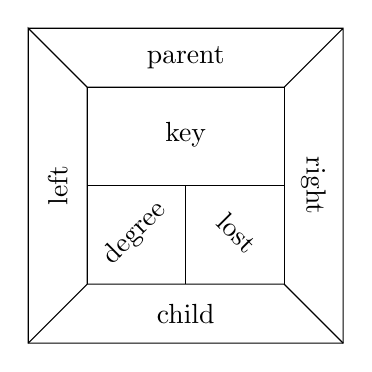
\begin{tikzpicture}[]

\draw[-](0,0)--++(4,0)--++(0,-4)--++(-4,0)--++(0,4)--++(0.75,-0.75)
--++(2.5,0)--++(0.75,0.75);
\draw[-](0.75,-0.75)--++(0,-2.5)--++(-0.75,-0.75);
\draw[-](0.75,0.75-4)--++(2.5,0)--++(0.75,-0.75);
\draw[-](-0.75+4,-4+0.75)--++(0,2.5);
\draw[-](0.75,-2)--++(2.5,0);
\draw[-](0.75+2.5/2,-4+0.75)--++(0,2.5/2);

\node at(2,-0.75/2){parent};
\node at(0.75/2,-2){\rotatebox{90}{left}};
\node at(4-0.75/2,-2){\rotatebox{270}{right}};
\node at(2,-4+0.75/2){\rotatebox{0}{child}};
\node at(2.65,-2.6){\rotatebox{315}{lost}};
\node at(4-2.65,-2.6){\rotatebox{45}{degree}};
\node at(2,-2+0.65){\rotatebox{0}{key}};
\end{tikzpicture}
\end{minipage}
\begin{minipage}{0.7\textwidth}
	Zugehöriger Baum:\\\up\up
	\usetikzlibrary{positioning,arrows}

\begin{tikzpicture}[every edge/.style={draw,->,>=stealth}]
\newcommand{\phan}[1]{\node(#1)[draw,circle] at(#1){\phantom{1}};}
\node (8-1) at (0,0) {8};
\phan{8-1}
\node (2) [right=of 8-1,xshift=1.25cm] {2};
\phan{2}
\node (3) [right=of 2,xshift=0cm] {3};
\phan{3}
\node (5) [right=of 3,xshift=.5cm] {5};
\phan{5}
\foreach \name/\position/\of/\shift/\out/\s in {12-1/below left/8-1/0.5/12/-0.1,
12-2/below/8-1/0/12/0,
9/below right/8-1/0/9/-0.1,
16/below/12-2/0/16/0,
10/below left/9/1/10/-0.1,
12-3/below right/9/-1/12/-0.1,
13/below/12-3/0/13/0,
4/below/3/0/4/0,
6-1/below left/5/1/6/-0.1,
6-2/below right/5/-1/6/-0.1,
8-2/below/6-2/0/8/0
}{
	\node (\name) [\position=of \of,xshift=\shift cm,yshift=\s cm,yshift=0.5cm] {\out};
	\phan{\name}
}
\foreach \x/\y in {12-1/8-1,12-2/8-1,9/8-1,16/12-2,10/9,12-3/9,13/12-3,4/3,6-1/5,6-2/5,8-2/6-2}{
	\draw(\x)edge(\y);
}
\foreach \x/\y in {8-1/2,2/3,3/5,12-1/12-2,12-2/9,10/12-3,6-1/6-2}{
	\draw[dashed,<->,>=stealth](\x)to(\y);
}

\foreach \x/\y/\out in {8-1/5/35,12-1/9/325,10/12-3/330,6-1/6-2/330}{
	\draw[dashed,<->,>=stealth](\x)to[out=\out, in=180-\out](\y);
}

\foreach \x/\y/\out/\in in {8-1/12-1/180/270-180,12-2/16/250/-250,9/10/270/35,12-3/13/290/-290,3/4/290/-290,5/6-1/270/40,6-2/8-2/290/-290}{
	\draw[->,color=red,>=stealth](\x)to[out=\out, in=\in](\y);
}
\node (min)[above=of 2,yshift=-0.65cm] {\textit{min}};
\draw(min)edge(2);
\end{tikzpicture}
\end{minipage}\\\ \\\ \\\ \\